\documentclass{beamer}
\usepackage[export]{adjustbox}
\usepackage[frenchb]{babel}
\usepackage[T1]{fontenc}
\usepackage[utf8]{inputenc}
\usepackage{listings}
\usepackage{fancyvrb}
\usetheme{Warsaw}

\title[Linux Embarqué]{Découverte de Linux Embarqué}
\author{maxime.chevallier@smile.fr}
\date{09 septembre 2016}
\institute{Smile / Open Wide Ingénierie}
\begin{document}

% Afficher plan à chaque section
\AtBeginSection[]{
	\begin{frame}
		\tableofcontents[currentsection, hideallsubsections]
	\end{frame}
}
\beamertemplatenavigationsymbolsempty{} % /o\ Pas de symboles de nav

% Numeros de slides
\addtobeamertemplate{navigation symbols}{}{%
    \usebeamerfont{footline}%
    \usebeamercolor[fg]{footline}%
    \hspace{1em}%
    \insertframenumber/\inserttotalframenumber
}
\setbeamercolor{footline}{fg=blue}
\setbeamerfont{footline}{series=\bfseries}
\setbeamertemplate{caption}{\raggedright\insertcaption\par}
\setbeamerfont{caption}{size=\tiny}
    \begin{frame}

	\titlepage

    \end{frame}

\begin{frame}
Intro
\end{frame}

\begin{frame}
\tableofcontents
\end{frame}

\section{Système embarqué}
\begin{frame}[t]
	\center{\huge{Système embarqué}}
	\begin{columns}
	\begin{column}[t]{0.45\linewidth}
		\begin{figure}
			\includegraphics<2->[height=2.5cm]{img/raspi.jpg}
			\uncover<2->{\caption{Raspberry pi 2}}
		\end{figure}
	\end{column}
	\begin{column}[t]{0.45\linewidth}
		\begin{figure}
			\includegraphics<3->[height=2.5cm]{img/arduino.jpg}
			\uncover<3->{\caption{Arduino UNO}}
		\end{figure}
	\end{column}
	\end{columns}
	\uncover<4->{\center{Pas des systèmes embarqués :(}}
\end{frame}
\begin{frame}[t]
	\center{\huge{Système embarqué}}
	\begin{columns}
	\begin{column}[t]{0.30\linewidth}
		\begin{figure}
			\includegraphics<2->[height=2.5cm]{img/roomba.jpg}
			\uncover<2->{\caption{aspirateur du futur}}
		\end{figure}
	\end{column}
	\begin{column}[t]{0.30\linewidth}
		\begin{figure}
			\includegraphics<3->[height=2.5cm]{img/tesla.jpg}
			\uncover<3->{\caption{voiture du futur}}
		\end{figure}
	\end{column}
		\begin{column}[t]{0.30\linewidth}
		\begin{figure}
			\includegraphics<4->[height=2.5cm]{img/router.jpg}
			\uncover<4->{\caption{routeur normal}}
		\end{figure}
	\end{column}
	\end{columns}
	\uncover<5->{\center{Systèmes embarqués :)}}
\end{frame}
% C'est quoi ?
\subsection{Contraintes}
\begin{frame}[t]
	\center{\huge{Contraintes}}
	\begin{block}<1->{Coûts matériels}
		\begin{itemize}
			\item Processeur
			\item Mémoire(s)
			\item Périphériques
		\end{itemize}
	\end{block}
	\begin{block}<2->{Coûts logiciels}
		\begin{itemize}
			\item Licenses ?
			\item Développements spécifiques ?
			\item Expertise ou support externe ?
			\item Evolution du produit ?
		\end{itemize}
	\end{block}
\end{frame}


\begin{frame}[t]
	\begin{block}<1->{Microcontrolleur}
		\begin{columns}[t]
			\begin{column}[T]{0.25\textwidth}
				\begin{figure}
					\includegraphics<1->[width=2.2cm]{img/atmega.jpg}
					\uncover<1->{\caption{Atmel ATMega 328}}
				\end{figure}
			\end{column}
			\begin{column}{0.70\textwidth}
				\begin{itemize}
					\item<2-> 1\euro50 / pièce
					\item<2-> 1 Cœur AVR 8bits @ 20 MHz
					\item<2-> 2 Ko RAM, 32 Ko Progmem
					\item<2-> I2C, SPI, UART
				\end{itemize}
			\end{column}
		\end{columns}
	\end{block}
	\begin{block}<3->{Microprocesseur}
		\begin{columns}[t]
			\begin{column}[T]{0.25\textwidth}
				\begin{figure}
					\includegraphics<3->[width=2.5cm]{img/imx.jpg}
					\uncover<3->{\caption{NXP iMX6 Quad}}
				\end{figure}
			\end{column}
			\begin{column}{0.70\textwidth}
				\begin{itemize}
					\item<4-> 36\euro / pièce
					\item<4-> 4 Cœurs ARM 32 bits @ 1GHz
					\item<4-> 256 Ko RAM, 96 Ko boot ROM
					\item<4-> DDR3, SDIO, eth, USB, HDMI, PCIe\dots
				\end{itemize}
			\end{column}
		\end{columns}
	\end{block}
\end{frame}

\begin{frame}[t]
	\center{\huge{Contraintes}}
	\begin{block}{Performances}
		\begin{itemize}
			\item Latences : Temps réel
			\item Temps de boot
			\item Capacité de calcul
		\end{itemize}
	\end{block}
	\begin{block}<2->{Environnement}
		\begin{itemize}
			\item Durabilité
			\item Environnement physique hostile
			\item Consommation
			\item Normes ( Radio, GPS )
		\end{itemize}
	\end{block}
\end{frame}

\begin{frame}
	\center{\huge{OS Temps-réel libres}}
	\begin{block}<2->{Contiki}
		\begin{columns}
		\begin{column}{0.50\textwidth}
		\begin{itemize}
			\item Orienté Networking et IoT
			\item Petite emprunte mémoire
			\item Riche en fonctionnalités
		\end{itemize}
		\end{column}
		\begin{column}{0.30\textwidth}
			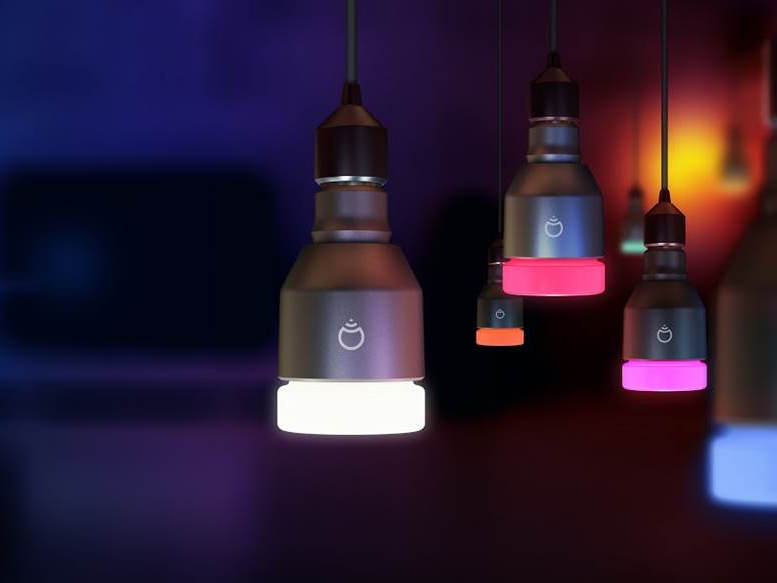
\includegraphics[height=2cm]{img/amp.jpg}
		\end{column}
		\end{columns}
	\end{block}
	\begin{block}<3->{freeRTOS}
		\begin{columns}
			\begin{column}{0.50\textwidth}
				\begin{itemize}
					\item Très petit
					\item Beaucoup d'architectures
					\item Éprouvé dans l'industrie
				\end{itemize}
			\end{column}
			\begin{column}{0.20\textwidth}
				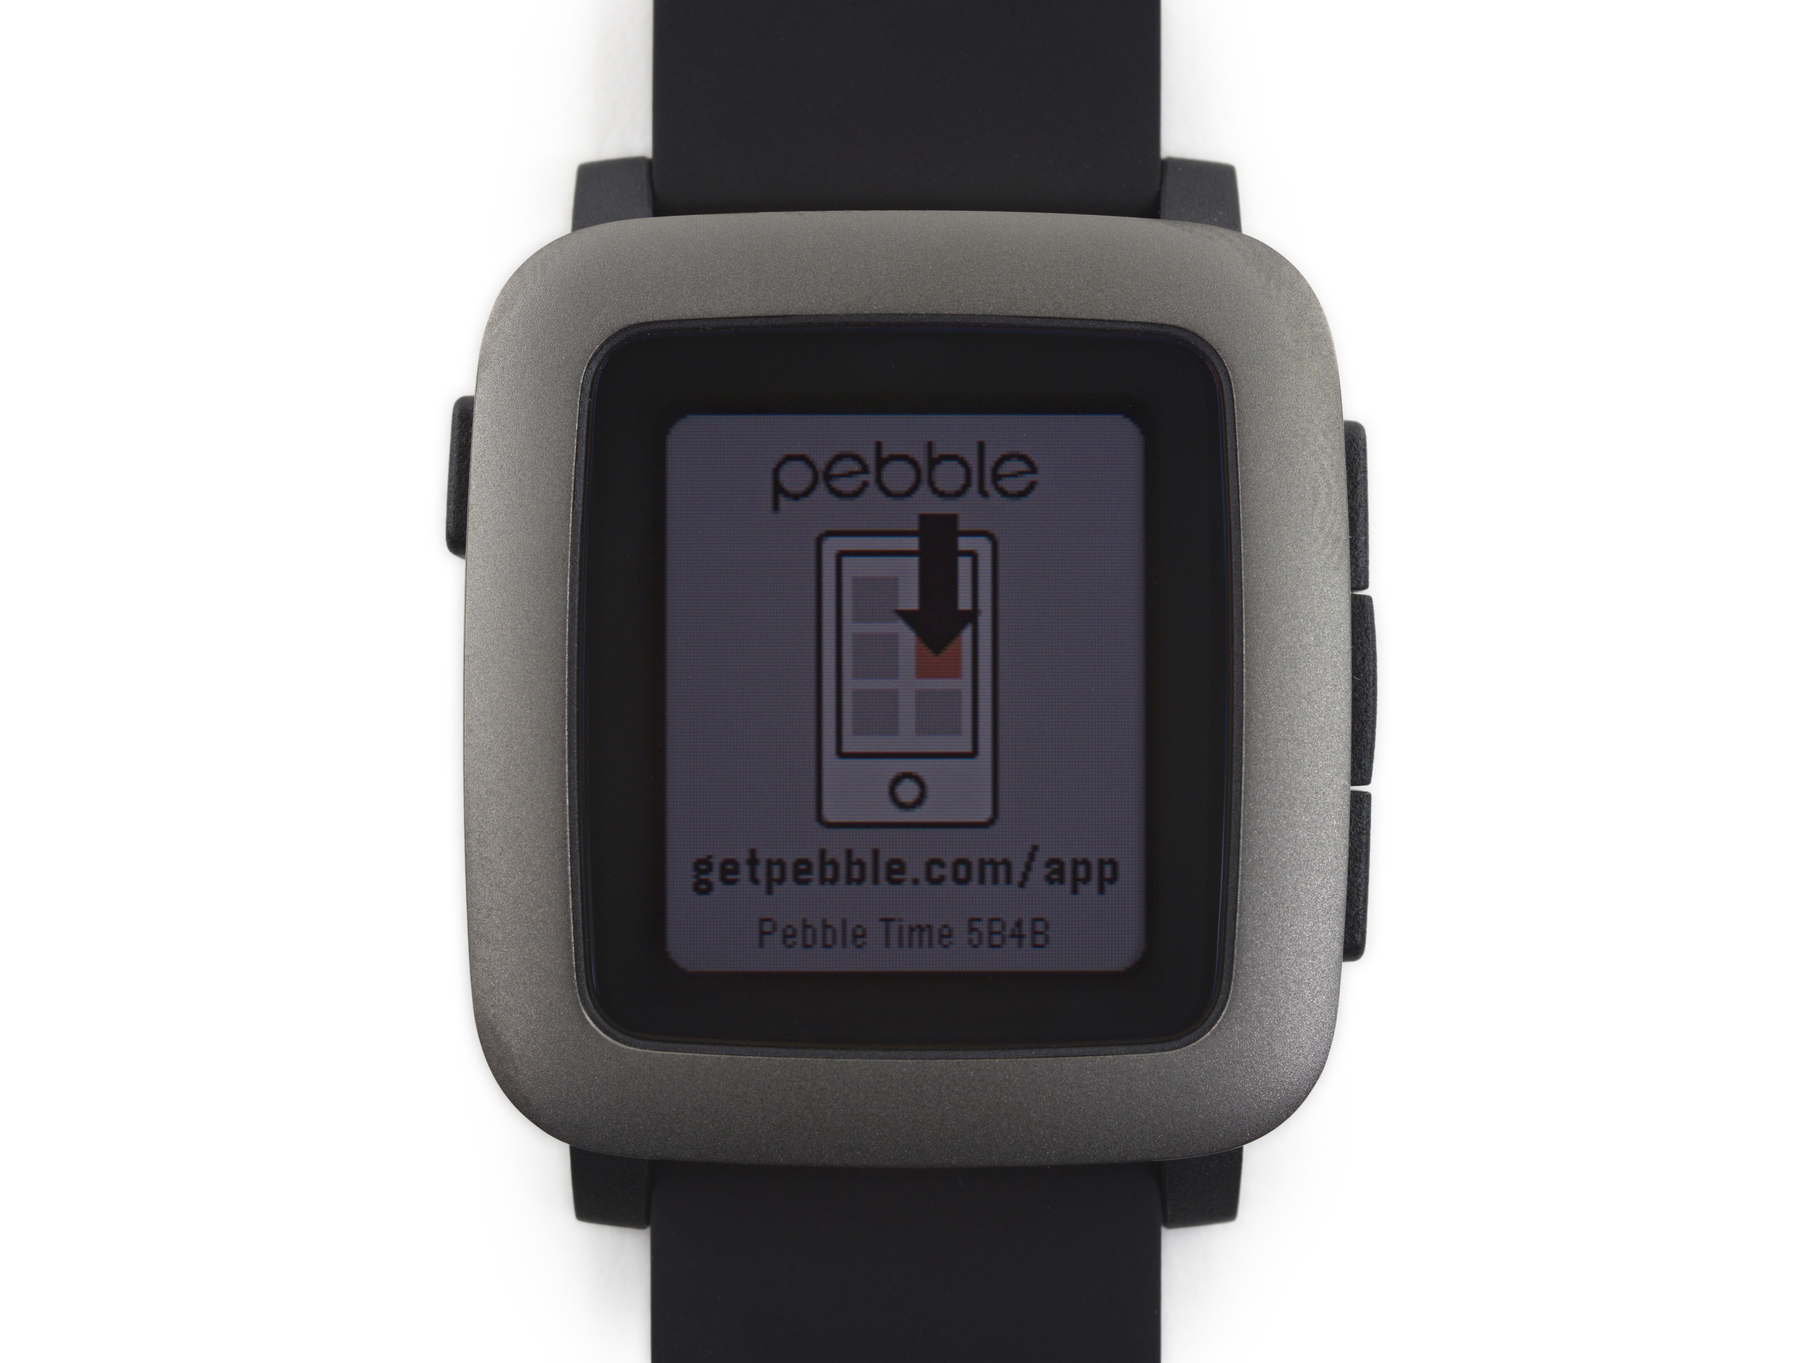
\includegraphics[height=2cm]{img/pt.jpg}
			\end{column}
			\begin{column}{0.20\textwidth}
				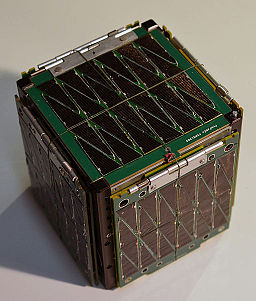
\includegraphics[height=2cm]{img/cubesat.jpg}
			\end{column}
		\end{columns}
	\end{block}
\end{frame}


% schéma
\section{Kernel}
\begin{frame}
	\center{\huge{Noyau}}
	\begin{minipage}[t]{0.45\linewidth}
		\begin{figure}
			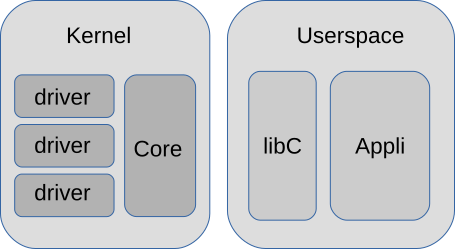
\includegraphics[height=5cm]{img/arch_linux_full.png}
			 \caption{kernel}
		\end{figure}
	\end{minipage}
	\begin{minipage}[t]{0.45\linewidth}
		\begin{itemize}
			\item Gère le matériel
			\item Gère les ressources
			\item Implémente certains protocoles
			\item Couche d'abstraction
			\item Isolé de l'espace utilisateur
			\item Composant critique
		\end{itemize}
	\end{minipage}

\end{frame}
\begin{frame}
	\center{\huge{Linux}}
	\begin{itemize}
		\item Beaucoup d'architectures
		\item Beaucoup de périphériques
		\item Beaucoup de fonctionnalités
		\item Communauté active
		\item Entièrement configurable
		\item Libre
		\item Documenté
		\item Polyvalent
	\end{itemize}
	\begin{block}{Variantes}
		\begin{itemize}
			\item Temps réeel : Preempt-RT, xenomai
			\item Microcontrolleur : uCLinux
			\item Sécurité : SELinux, grsecurity
		\end{itemize}
	\end{block}
\end{frame}
% choix de la version
\subsection{Drivers}
\begin{frame}
	\center{\huge{Drivers}}
	\begin{itemize}
		\item Support d'un périphérique
		\item Support d'un protocole
		\item Libre ou Propriétaire
	\end{itemize}
	\begin{block}{Kernel module}
		\item Extension du kernel
		\item Intégration statique ou dynamique
		\item Lié à une version du kernel
		\item Gestion des dépendances
	\end{block}
\end{frame}
% drivers, support
\subsection{Configuration}
\begin{frame}
		\begin{itemize}
			\item Choix des drivers
			\item Choix des fonctionnalités
			\item Options de debug
			\item Options d'optimisation
		\end{itemize}
	\begin{block}{Kconfig}
		\begin{itemize}
			\item Plusieurs UI
			\item Dépendances entre options
			\item Génère un fichier de conf
		\end{itemize}
	\end{block}

\end{frame}
% choix des options : selon matos, contraintes

% Schema
\section{Userspace}
	\begin{frame}
		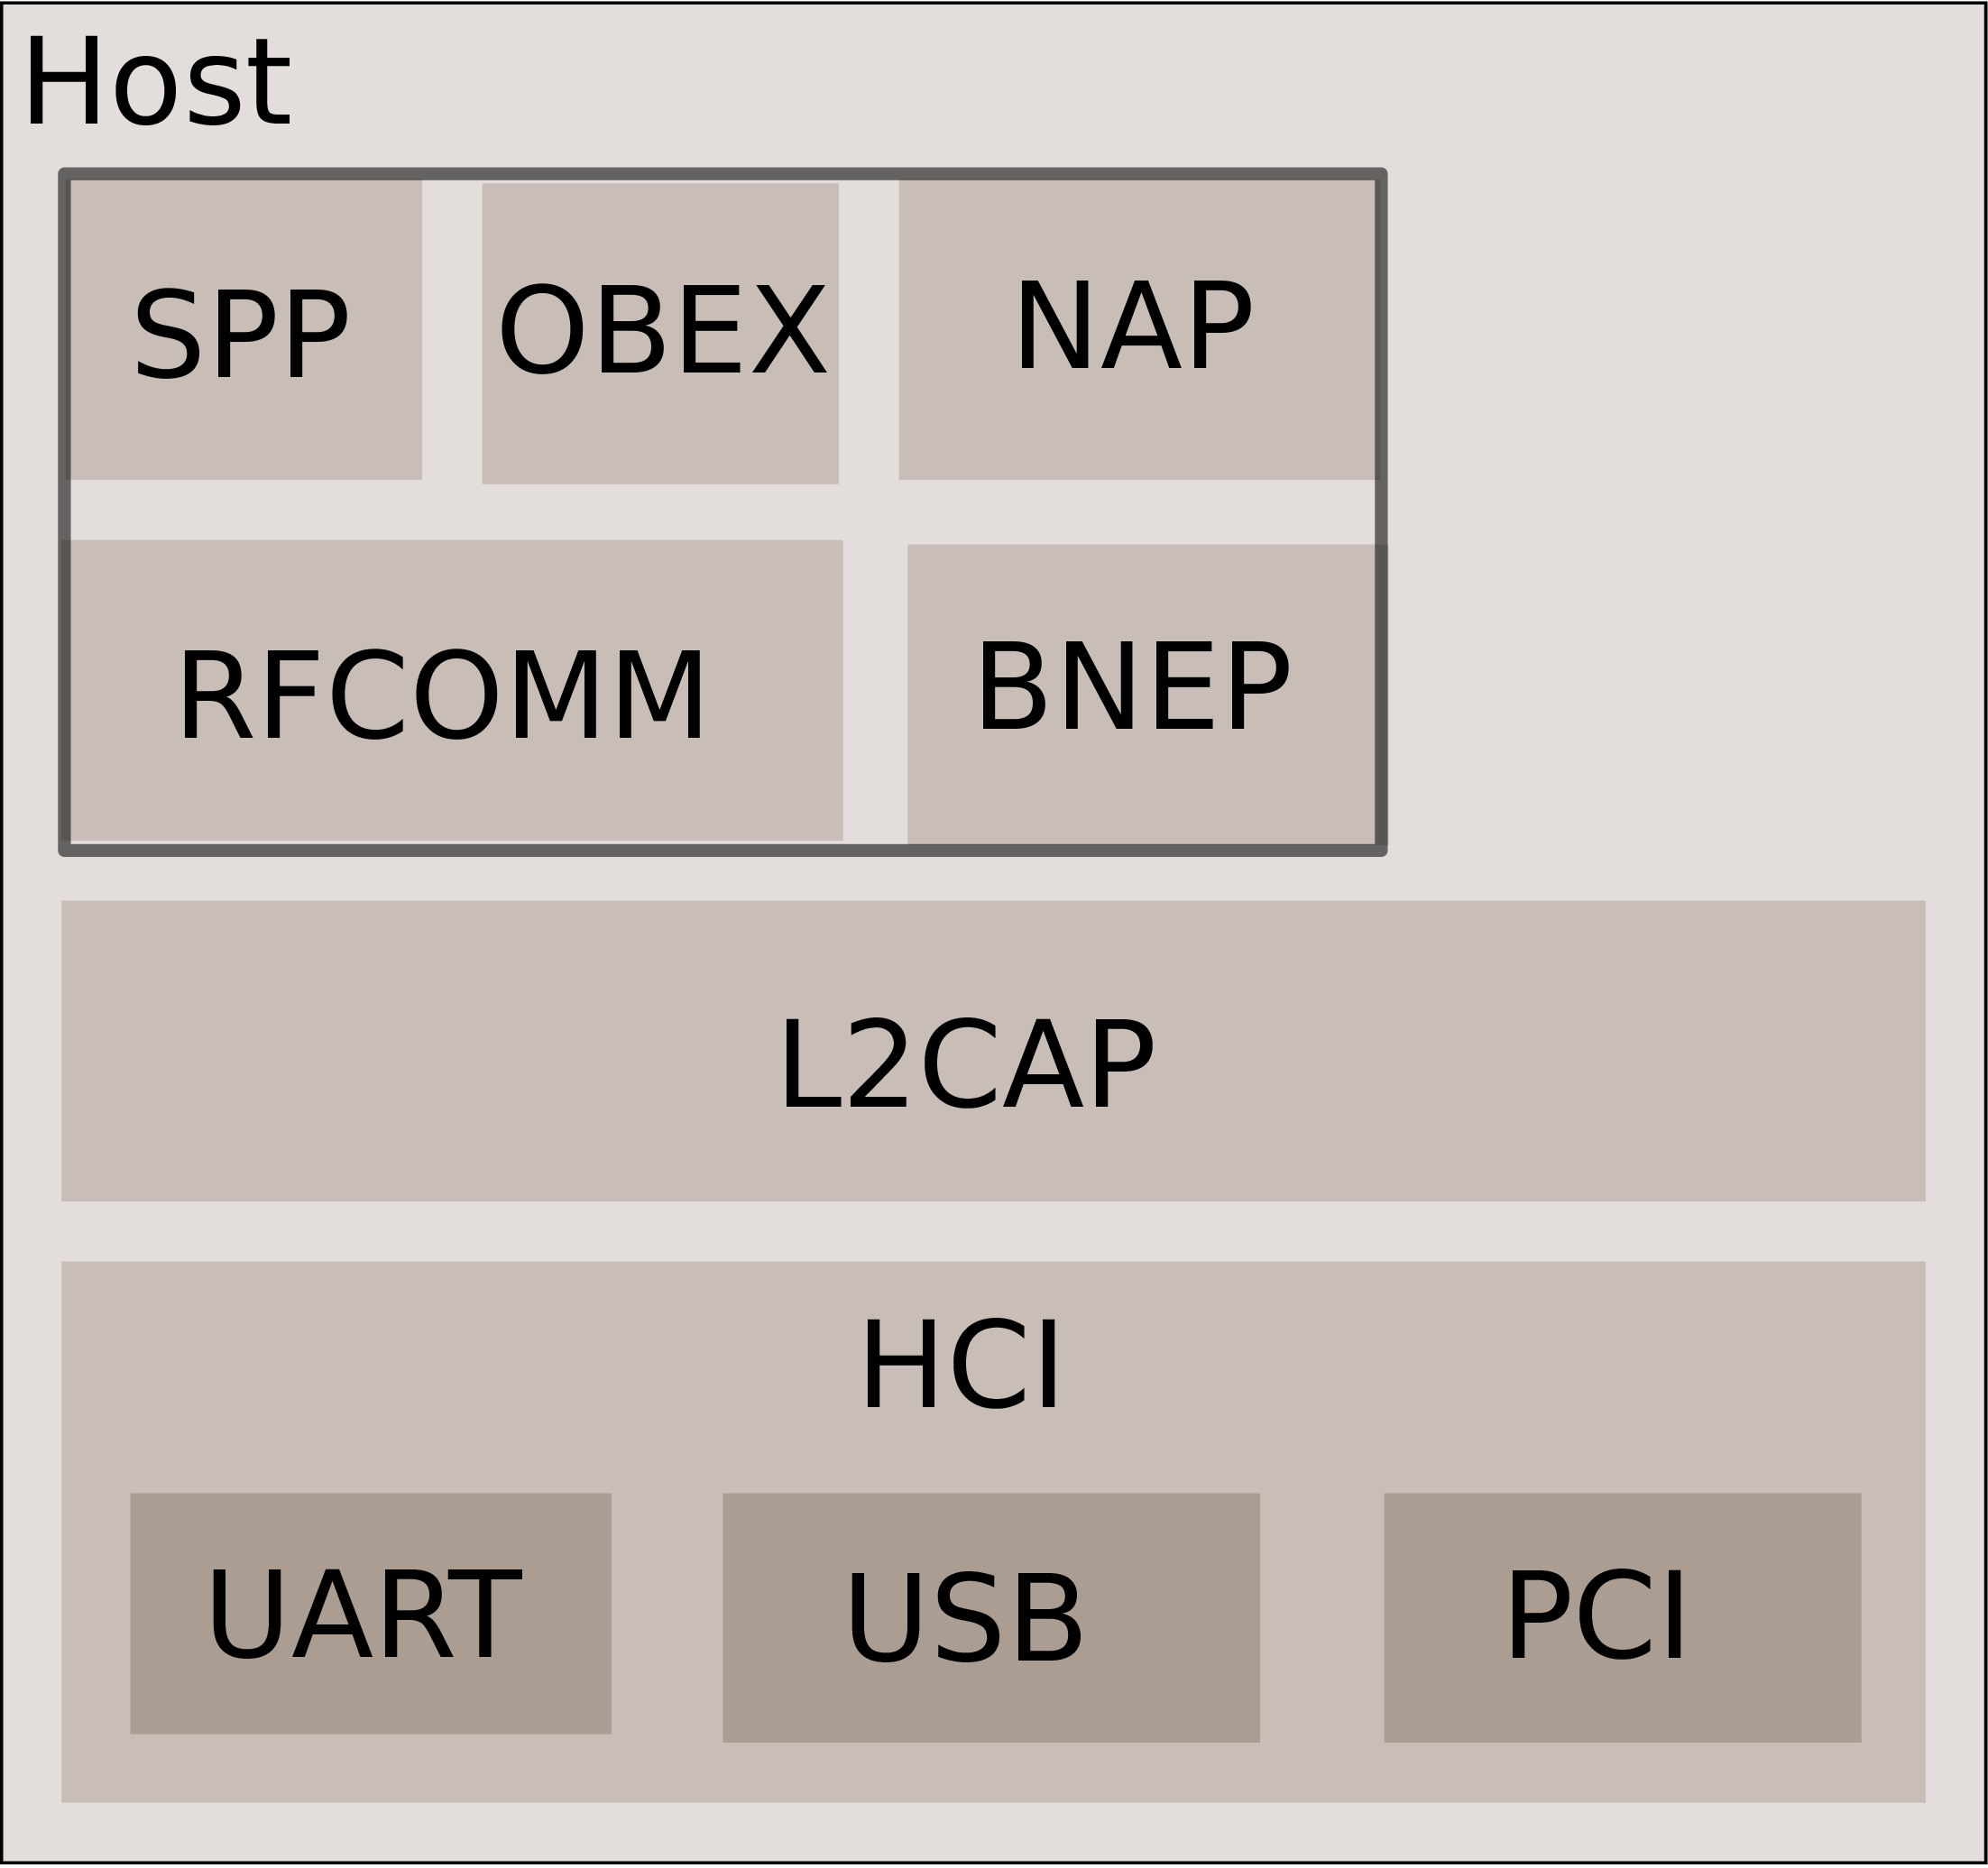
\includegraphics[height=5cm]{img/arch_log_all.png}
		\caption{kernel + userspace}
	\end{frame}
	\begin{frame}
		\center{\huge{Système d'init}}
		\begin{itemize}
			\item Premier processus lancé
			\item Lance les autres processus
			\item Influe sur le temps de boot
		\end{itemize}
		\begin{block}{SysV init}
			\begin{itemize}
				\item Scripts
				\item Peu de parallélisation
			\end{itemize}
		\end{block}
		\begin{block}{Systemd}
			\begin{itemize}
				\item Fichiers de configuration
				\item Parallélisation et dépendances
				\item Plus complexe
			\end{itemize}
		\end{block}
	\end{frame}

\subsection{libC}
% choix de la libC
\subsection{Outils}
% choix des libs
\subsection{Librairies}
% choix des outils ( busybox, vrai outils )

\section{Bootloader}
%role
\begin{frame}[t]
	%schema boot + kernel
	\begin{columns}[t, totalwidth=\textwidth]
		\begin{column}[t]{0.40\linewidth}
		\begin{figure}
			\includegraphics<1-5>[width=4cm]{img/boot_bl.png}
			\includegraphics<6>[width=4cm]{img/boot_bl_kern.png}
			\includegraphics<7->[width=4cm]{img/boot.png}
			\caption{boot sequence}
		\end{figure}

	\end{column}
		\begin{column}[t]{0.45\linewidth}
	\begin{block}{Boot Sequence}
		\begin{itemize}
			\item<1-> Power On
			\item<2-> Bootloader chargé
			\item<3-> Bootloader exécuté
			\item<4-> Init matériel
			\item<5-> Noyau chargé
			\item<6-> Noyau exécuté
			\item<7-> /sbin/init appelé
		\end{itemize}
	\end{block}
	\end{column}
	\end{columns}
\end{frame}
%U Boot
\begin{frame}
	\center{\huge{Das U-Boot}}

\end{frame}

% Barebox
\begin{frame}
	\center{\huge{Barebox}}
\end{frame}


\section{Build system}
% schema
\subsection{Buildroot}
% buildroot
\subsection{Yocto}
% yocto

% interet du libre
% conclu


\end{document}
